\documentclass[article]{whu-bachelor-style}
\usepackage{float}
\usepackage{array}
\usepackage{dsfont}

% 算法伪代码中文关键词
\SetKwInput{KwIn}{输入}
\SetKwInput{KwOut}{输出}
\SetKw{KwRet}{返回}
\SetKw{KwInit}{初始化}
\newcommand{\sys}{ProtoPurify}

\begin{document}
%%----------- 封面部分 ----------- %%
  \ctitle{面向大语言模型后门防御即服务的原型表示净化方法研究}
  \cschool{国家网络安全学院}
  \cmajor{信息安全专业}
  \cauthor{高嘉鑫}
  \cnumber{2022302191146}
  \cadvisor{王骞\quad 教授}
  \cdate{二〇二六年四月}

  \maketitlepage            % 封面
  \makestatement            % 申明

%%----------- 前言部分 ----------- %%
  % 中英文摘要
\phantomsection
\pagenumbering{Roman}
\addcontentsline{toc}{chapter}{摘\hspace{1em}要}

\begin{cnabstract}{大语言模型；后门攻击；后门净化；后门防御即服务；原型表示；权重空间}

大语言模型（LLMs）已被广泛部署于安全敏感型应用场景，但仍面临后门攻击的严重威胁。现有后门防御方法难以在"后门防御即服务"（Backdoor Defense-as-a-Service，BDaaS）场景下实际落地，原因在于这些方法通常依赖不切实际的先验信息（如下游干净数据、已知触发器或目标输出），且缺乏针对不同后门模型的可复用、可扩展净化能力。

本文提出后门净化框架ProtoPurify，在极少先验假设的条件下通过参数编辑实现高效后门净化。ProtoPurify首先从干净模型与后门模型的参数差值中构建后门向量池，通过聚合操作生成候选原型向量，并利用余弦相似度匹配为目标后门模型选择最优原型。随后，该方法通过逐层原型对齐分析检测边界层，并在候选层中抑制与原型对齐的参数分量，从而在最小化良性性能损失的前提下实现精细化的后门行为净化。作为面向BDaaS的服务化原语，ProtoPurify原生支持可复用性、可定制化、可解释性和运行时高效性四大核心特性。

在多种大语言模型上针对分类与生成任务的实验表明，ProtoPurify在面对6种多样化攻击（包括单触发器、多触发器和无触发器后门设置）时，始终优于6种代表性防御方法。ProtoPurify能够将攻击成功率（ASR）降低至10\%以下，部分情况下甚至低至1.6\%，同时干净数据准确率（CDA）损失不超过3\%。此外，ProtoPurify在未见数据集和未知攻击类型上具备良好的泛化能力，对自适应后门变体具有较强的鲁棒性，且在无后门模型上能够保持稳定性能。

\end{cnabstract}
\newpage

\phantomsection
\addcontentsline{toc}{chapter}{ABSTRACT}

\begin{enabstract}{Large Language Model; Backdoor Attack; Backdoor Purification; Defense-as-a-Service; Prototype Representation; Weight Space}

Large language models (LLMs) are increasingly deployed in security-sensitive applications, yet remain vulnerable to backdoor attacks. However, existing backdoor defenses are difficult to operationalize for Backdoor Defense-as-a-Service (BDaaS), as they require unrealistic side information (e.g., downstream clean data, known triggers/targets, or task domain specifics), and lack reusable, scalable purification across diverse backdoored models.

In this paper, we present ProtoPurify, a backdoor purification framework via parameter edits under minimal assumptions. ProtoPurify first builds a backdoor vector pool from clean and backdoored model pairs, aggregates vectors into candidate prototypes, and selects the most aligned candidate for the target model via cosine similarity matching. ProtoPurify then identifies a boundary layer through layer-wise prototype alignment and performs targeted purification by suppressing prototype-aligned components in the affected layers, achieving fine-grained mitigation with minimal impact on benign utility. Designed as a BDaaS-ready primitive, ProtoPurify supports reusability, customizability, interpretability, and runtime efficiency.

Experiments across various LLMs on both classification and generation tasks show that ProtoPurify consistently outperforms 6 representative defenses against 6 diverse attacks, including single-trigger, multi-trigger, and triggerless backdoor settings. ProtoPurify reduces the attack success rate (ASR) to below 10\%, and even as low as 1.6\% in some cases, while incurring less than a 3\% drop in clean data accuracy (CDA). Furthermore, ProtoPurify generalizes effectively to held-out datasets and previously unseen backdoor attacks, remains robust to adaptive backdoor variants, and preserves stability on non-backdoored models.

\end{enabstract}
\newpage
  % 摘要
  \makecontents             % 目录

%%----------- 主体部分 ----------- %%
  % 第一章：绪论

\chapter{绪论}

\section{研究背景与意义}

近年来，以GPT系列\cite{brown2020gpt3,achiam2023gpt4}和Llama系列\cite{dubey2024llama3}为代表的大语言模型（Large Language Models，LLMs）在自然语言处理领域取得了突破性进展，在文本生成、机器翻译、问答系统、情感分析等多种任务上展现出卓越性能。这些模型凭借其强大的泛化能力，已在金融风控、医疗辅助、智能教育等安全敏感型行业实现了广泛部署，显著提升了相关领域的自动化水平和用户体验。

然而，大语言模型的广泛应用也带来了前所未有的安全挑战。\textbf{后门攻击}（Backdoor Attack）是一种尤为隐蔽且危险的训练期威胁。攻击者通过污染训练数据或直接修改模型参数，在模型中植入隐藏的触发器（Trigger），使模型在正常输入上表现如常，但一旦输入包含特定触发器，模型便会输出攻击者预设的恶意结果。后门攻击难以被检测的根本原因在于：触发器形式多样（可以是特定词语、句法结构、语义模式等），且对防御方而言通常是完全未知的；此外，大语言模型的庞大参数规模和复杂的参数化方式使得后门行为深埋于高维隐空间之中，难以被现有方法准确定位和消除。

随着大模型训练成本的急剧上升，模型的开发、微调乃至部署过程日益外包给第三方服务提供商，这使得模型在供应链各环节均面临被植入后门的风险。在此背景下，一种新型安全服务范式——\textbf{后门防御即服务}（Backdoor Defense-as-a-Service，BDaaS）应运而生。在这种范式下，模型所有者可在模型部署前将其提交至专业安全平台，由平台对模型进行后门净化，从而降低将受损模型投入生产的风险。这一设想与业界已有的商业化安全服务（如TrojAI Detect、CalypsoAI推理平台）的运作模式高度契合。

然而，现有后门防御方法在实际落地BDaaS场景时面临两大核心瓶颈。

\textbf{其一，对先验信息的强依赖。}许多方法需要目标任务的干净数据集、已知的触发器或目标输出信息，乃至任务领域信息。然而在通用大模型的服务化场景中，这些信息往往不可获取或涉及用户隐私，难以作为服务的预设条件。

\textbf{其二，缺乏可复用性。}现有方法通常针对每个受损模型独立进行净化，无法将之前积累的知识和防御组件复用到后续模型的净化中，严重制约了服务化平台的规模化能力和经济性。

鉴于上述挑战，本文提出ProtoPurify方法，通过在极少先验假设的条件下构建和利用后门原型向量，实现跨数据集、跨任务的通用后门净化，为大语言模型后门防御即服务提供了一种可行的技术路径。

\section{国内外研究现状}

\subsection{后门攻击研究}

后门攻击在深度学习领域已有较为深入的研究。根据触发器设计方式的不同，现有攻击方法大致分为三类：

\textbf{单触发器后门攻击}（Single-trigger Backdoor Attack）是最基础的攻击形式，使用单一固定触发器操控模型输出。Kurita等人\cite{kurita2020weight}针对BERT模型提出了基于稀有词的后门攻击；BadEdit\cite{li2024badedit}通过直接修改模型权重植入后门，无需污染训练数据。此类攻击依赖显式词汇线索，在一定程度上可被简单的异常词检测防御识别。

\textbf{多触发器后门攻击}（Multi-trigger Backdoor Attack）将触发器分散至多个输入部分，仅当所有触发器同时出现时才激活恶意行为，显著提高了攻击隐蔽性。复合后门攻击（CBA）\cite{huang2023cba}将触发器散布于用户查询与系统指令等不同提示片段；双触发器后门攻击\cite{hou2024dual}要求特定句法模板与虚拟语气模式同时出现方可激活，进一步增强了抗检测能力。

\textbf{无触发器后门攻击}（Triggerless Backdoor Attack）不依赖显式触发器字符串，而是利用语义或句法上的隐蔽条件激活恶意行为。虚拟提示注入（VPI）\cite{yan2024vpi}通过语义级触发器操控模型输出；分布式触发器后门攻击（DTBA）\cite{hao2024dtba}则将触发器分散于多轮对话之中，此类攻击对传统检测方法构成了更严峻的挑战。

\subsection{后门防御研究}

针对后门攻击的防御方法主要分为检测和净化两大方向。净化方法因能直接消除后门行为并恢复模型的可部署状态而更具实用价值，可进一步细分为以下四类：

\textbf{基于微调的方法}通过在干净数据上重新训练覆盖后门行为，代表方法包括NAD（神经注意力蒸馏）\cite{li2021nad}和W2SDefense\cite{yang2022w2sdefense}等。此类方法计算代价通常较高，且对高级后门攻击效果有限。

\textbf{基于剪枝的方法}通过剪除编码后门行为的参数子集实现净化，代表方法包括Fine-Pruning\cite{liu2018finepruning}、PURE\cite{zhu2024pure}和Obliviate\cite{li2024obliviate}等。这类方法依赖干净数据集识别需要剪除的参数，同样存在先验信息依赖问题。

\textbf{基于参数编辑的方法}将后门视为模型权重中的局部关联，通过直接修改小部分参数消除，代表方法包括ROME\cite{meng2022rome}和MEMIT\cite{meng2023memit}等。此类方法要求防御方知晓触发的不当行为，对未知或语义触发器效果有限。

\textbf{基于嵌入的方法}{\sloppy 
在表示空间而非直接在权重中运作，代表方法包括BEEAR\cite{zeng2024beear}和CROW\cite{min2024crow}等。BEEAR通过对抗性操控嵌入空间中的后门方向消除后门；CROW通过内部一致性正则化实现稳定的跨层表示。
\par}

上述方法虽在特定设置下取得了一定效果，但普遍存在对先验信息的强依赖或缺乏可复用机制等问题，难以直接适用于BDaaS场景。

\subsection{权重空间表示研究}

近期研究揭示了模型行为可以通过权重空间中的向量来捕获和操控这一重要规律。任务向量\cite{ilharco2023taskv}将模型在微调前后的参数差值形式化为编码特定任务能力的向量，这些向量具有近似线性的代数性质，可通过加减运算实现能力的组合或消除。模型合并（Model Soups）\cite{wortsman2022soups}等方法进一步证明，独立微调模型的权重平均可提升性能和鲁棒性。这些发现为本文提出的基于权重空间的后门净化方法提供了重要的理论支撑。

\section{主要研究内容与贡献}

本文围绕面向大语言模型后门防御即服务的核心需求，提出了基于原型表示的后门净化方法ProtoPurify，核心思想源于以下实证发现：不同后门攻击在模型参数空间中往往引发相关的参数变化，这意味着存在一个共享的恶意后门"原型"，可被识别和利用以实现通用净化。

本文的主要贡献如下：

\begin{enumerate}[leftmargin=2em]
    \item \textbf{提出ProtoPurify净化框架。}在极少先验假设（无需了解触发器、训练数据或下游任务信息）的条件下，通过构建原型向量实现后门净化，原生支持可复用性、可定制化、可解释性和运行时高效性，是面向BDaaS场景的实用防御框架。

    \item \textbf{构建端到端权重空间净化流程。}该流程包含四个核心阶段：通过配对模型模拟提取后门向量（阶段一）、通过聚合操作构建候选原型（阶段二）、通过逐层对齐分析检测边界层（阶段三），以及通过抑制原型对齐分量实现可控净化（阶段四）。

    \item \textbf{开展系统性实验验证。}在Llama3-8B和Mistral-7B两种主流大语言模型上，针对分类与生成任务进行广泛实验，结果表明ProtoPurify在面对单触发器、多触发器和无触发器后门时，净化效果与模型效用的综合表现始终优于6种代表性防御基线，同时对自适应后门攻击具有较强鲁棒性，且在无后门模型上不造成性能损失。
\end{enumerate}

\section{论文结构安排}

本文的结构安排如下：

\textbf{第一章}为绪论，介绍研究背景与意义、国内外研究现状、主要研究内容与贡献以及论文结构安排。

\textbf{第二章}为相关工作，系统梳理大语言模型的基础知识、后门攻击与防御的研究进展，以及权重空间表示的相关方法，为本文方法的提出奠定理论基础。

\textbf{第三章}为ProtoPurify方法，详细阐述威胁模型的定义、方法总体框架，以及后门模拟、原型构建、边界层检测和模型净化四个核心阶段的技术细节，并给出完整的算法伪代码。

\textbf{第四章}为实验与结论，介绍实验设置、与6种基线方法的全面对比结果、消融实验分析、面向BDaaS四大特性的分析、自适应攻击鲁棒性评估以及全文总结。

  % 第二章：相关工作

\chapter{相关工作}

\section{大语言模型}

大语言模型（Large Language Models，LLMs）是基于Transformer架构的深度学习模型，利用自注意力机制捕获序列内的复杂依赖关系，能够处理和生成类人文本。以GPT-3\cite{brown2020gpt3}、GPT-4\cite{achiam2023gpt4}、Llama 3\cite{dubey2024llama3}和Mistral\cite{jiang2023mistral}为代表的大语言模型在文本生成、机器翻译、对话系统等任务上展现出卓越性能，已在金融、医疗、教育等多个行业实现大规模应用。

大语言模型的训练通常包含预训练和微调两个阶段。

\subsection{预训练}

在预训练阶段，模型通过因果语言建模目标（Causal Language Modeling）\cite{vaswani2017attention}在大规模语料库上学习通用的语言表示，即最大化序列中下一个词元的条件概率：
\begin{equation}
L_{\text{causal}} = - \sum_{i=1}^{N} \log P(x_i \mid x_{<i}; \theta)
\end{equation}
其中$x_i$表示第$i$个词元，$x_{<i}$表示其前驱词元序列，$\theta$为模型参数。预训练过程的核心是自注意力机制，该机制通过计算查询、键和值矩阵之间的相似度来捕获词元间的关联：
\begin{equation}
\text{Attention}(Q, K, V) = \text{softmax}\!\left(\frac{QK^\top}{\sqrt{d_k}}\right)V
\end{equation}
其中$Q$、$K$、$V$分别为查询、键和值矩阵，$d_k$为键向量的维度。

\subsection{微调}

预训练完成后，模型通过在特定任务数据集上优化任务相关的损失函数（如交叉熵损失）进行微调\cite{hu2022lora}，以适应下游应用需求。此外，基于人类反馈的强化学习（RLHF）等对齐方法\cite{ouyang2022rlhf}通过引入源自人类评估的奖励信号，进一步使模型输出与人类偏好保持一致，广泛应用于对话系统等场景。

尽管大语言模型取得了显著进展，其在安全性方面仍存在严重隐患。本文重点关注后门攻击这一训练期威胁，旨在通过开发稳健的防御机制为大语言模型的安全部署提供保障。

\section{后门攻击}

后门攻击（Backdoor Attack）是一种隐蔽的训练期安全威胁，攻击者通过在训练数据中植入中毒样本或直接修改模型参数，使模型在接收含有特定触发器的输入时产生恶意输出，而在正常输入上保持与未受攻击模型相同的行为。随着大语言模型的广泛部署和对海量数据集的依赖，后门攻击已成为一个日益严峻的安全问题。根据触发器设计方式的不同，现有攻击方法分为以下三类。

\subsection{单触发器后门攻击}

单触发器后门攻击（Single-trigger Backdoor Attack）使用单一固定触发器（如特定词语序列或文本模式）操控模型输出。Kurita等人\cite{kurita2020weight}针对BERT模型提出了干净标签后门攻击，通过使用稀有触发词进行微调诱导攻击者选定的词元预测。BadEdit\cite{li2024badedit}则证明，单触发器后门同样可以通过模型编辑的方式植入——直接修改模型权重以建立触发器与目标行为之间的关联，无需污染训练数据。Qi等人\cite{qi2021hidden}使用预先指定的句法模板作为触发器，生成流畅的中毒输入并抵抗简单的词过滤防御。此类设计依赖显式词汇线索，在一定程度上可被简单的异常词检测防御识别。

\subsection{多触发器后门攻击}

多触发器后门攻击（Multi-trigger Backdoor Attack）将触发器分散至多个输入组件，仅当所有触发器同时出现时才激活恶意有效载荷，从而在提升隐蔽性的同时增强触发控制。Huang等人\cite{huang2023cba}提出的复合后门攻击（CBA）将触发器分散至不同的提示片段（如用户查询与系统指令），大幅降低了良性输入意外激活后门的概率。Hou等人\cite{hou2024dual}提出的双触发器文本后门攻击仅当特定句法模板和虚拟语气模式同时出现时才被激活，相比基于词元的触发器具有更强的隐蔽性。

\subsection{无触发器后门攻击}

无触发器后门攻击（Triggerless Backdoor Attack）不依赖显式触发器字符串，而是在看似正常的输入中嵌入隐蔽的激活条件。后门可以在语义层面被触发——特定的含义、意图或话题隐式充当触发器；也可以在句法层面被触发——特定的结构模式充当隐藏触发器。Yan等人\cite{yan2024vpi}针对指令微调的大语言模型提出了虚拟提示注入（VPI），通过语义触发器使模型表现得如同攻击者选定的虚拟提示被隐式追加，无需任何显式触发器字符串即可操控输出。Hao等人\cite{hao2024dtba}提出了分布式触发器后门攻击（DTBA），将场景级触发器分散于多轮对话之中，检测难度极高。此类攻击对传统触发器过滤防御方法构成了更严峻的挑战。

\section{后门防御}

后门防御方法主要分为检测（Detection）和净化（Purification）两大方向。检测方法旨在识别后门模型或含触发器的输入，但无法将受损模型恢复至可安全部署的状态。净化方法直接消除后门行为同时保留良性功能，更具实用价值。本文聚焦于后门净化，现有方法可分为以下四类。

\subsection{基于微调的防御}

基于微调的防御（Fine-tuning-based Defense）通过在良性数据上训练来抑制后门模型的恶意行为，同时保留干净性能。NAD（Neural Attention Distillation）\cite{li2021nad}采用基于蒸馏的微调策略，由干净教师模型引导后门学生模型在干净数据上匹配中间层的注意力表示。W2SDefense\cite{yang2022w2sdefense}通过训练小型干净教师模型并借助参数高效微调（如LoRA\cite{hu2022lora}）蒸馏至后门学生模型，在无需完整重训练的条件下实现高效的后门遗忘。然而，此类方法计算代价较高，对高级后门攻击效果有限，且依赖目标任务的干净数据集。

\subsection{基于剪枝的防御}

基于剪枝的防御（Pruning-based Defense）通过剪除或屏蔽编码后门行为的参数子集实现净化，代表方法包括Fine-Pruning\cite{liu2018finepruning}、PURE\cite{zhu2024pure}和Obliviate\cite{li2024obliviate}等。Fine-Pruning移除干净输入激活值较低的神经元（随后进行轻量微调）；PURE通过剪枝后门相关注意力头并归一化激活来抑制恶意行为；Obliviate针对PEFT场景中嵌入在LoRA适配器中的后门，通过干净探测统计检测可疑维度并选择性清零实现净化；Wanda\cite{sun2023wanda}作为轻量级净化基线，通过剪除激活感知重要性分数$|w| \cdot |a|$较低的权重实现净化。

\subsection{基于参数编辑的防御}

基于参数编辑的防御（Parameter-editing-based Defense）将后门视为嵌入在模型权重中的局部关联，通过直接修改小部分参数消除后门。ROME\cite{meng2022rome}通过对MLP层进行低秩更新重写局部关联，在防御方能够提供显式反事实对的情况下消除后门；MEMIT\cite{meng2023memit}将该范式推广至大规模多关联的高效重写。此类方法不引入推理开销，但假设触发的不当行为是可识别的且后门是充分局部化的，对未知或语义触发器效果有限。

\subsection{基于嵌入的防御}

基于嵌入的防御（Embedding-based Defense）在表示空间而非直接在模型权重中运作，核心直觉在于后门行为在嵌入空间中表现为异常方向。BEEAR\cite{zeng2024beear}通过对抗性操控嵌入表示来识别和消除指令微调大语言模型中的安全后门；CROW\cite{min2024crow}利用后门触发器引发异常逐层表示不稳定性的观察，在小型干净提示集上进行带内部一致性正则化器的轻量微调，无需触发器知识或干净参考模型。

然而，上述净化方法要么依赖不切实际的先验信息，要么缺乏可复用的净化机制，限制了其在BDaaS场景中的实用性。

\section{权重空间表示}

近期研究揭示了模型行为可以直接在权重空间中被捕获、表达和操控这一重要规律，为本文提出的后门净化方法奠定了理论基础。

\subsection{任务向量}

Ilharco等人\cite{ilharco2023taskv}将模型在微调前后的参数差值形式化为\textbf{任务向量}（Task Vector）：令$\tau = \theta_{\text{fine-tuned}} - \theta_{\text{base}}$，这些向量展现出近似线性的代数性质，可以被加减以组合行为，或取反以抑制特定能力。任务向量还支持类比迁移——令$\Delta_{A \to B} = \theta_B - \theta_A$，将其应用于另一个模型$\theta_C$可得：
\begin{equation}
\theta_D \approx \theta_C + \Delta_{A \to B}
\end{equation}
即使未在目标任务上进行训练，也能实现一定程度的能力迁移。这一发现表明，有意义的模型行为变化可以通过权重空间中的向量运算来捕获和迁移。

\subsection{模型合并}

Wortsman等人\cite{wortsman2022soups}提出的模型合并（Model Soups）框架证明，多个从同一基础模型独立微调得到的模型通常处于共享的低损失区域，对其权重取平均可以在不增加推理成本的情况下超越最佳单一检查点的性能，并提升鲁棒性和泛化能力。这一经验性发现表明，有意义的权重更新在参数空间中具有可组合性，模型行为可以通过轻量的权重运算被组合、迁移乃至部分消除。

此外，模型引导（Model Steering）的相关工作表明，高层行为可以通过紧凑的线性方向来控制。通过对比不同属性下的模型状态（如有毒vs.无害），可以提取出可作为行为控制器的方向向量，在推理时可用于执行诱导模型行为转变的表示编辑。

\subsection{对后门净化的启示}

上述研究共同揭示了一个关键洞见：模型行为可以被表达为权重空间中的向量，并可通过向量运算加以操控。如果良性微调行为可以被编码为任务向量并进行迁移，那么恶意的后门行为也应当可以被抽象为参数空间中的向量，并通过向量操作加以识别和消除。本文提出的ProtoPurify方法正是基于这一洞见，通过提取代表性的后门原型向量，并利用其在权重空间中抑制与之对齐的后门相关参数分量，实现通用后门净化。

  % 第三章：ProtoPurify方法

\chapter{ProtoPurify方法设计}

\section{威胁模型}

\subsection{防御方假设}

防御方运营一个BDaaS平台，负责对用户提交的可能含有后门的模型$M'$进行净化。防御方具有以下约束：
\begin{itemize}[leftmargin=2em]
    \item \textbf{无法访问私有训练数据}：防御方不知晓用于构建后门模型的原始私有训练数据，也无法观察内部训练过程。
    \item \textbf{无后门先验知识}：防御方不知晓后门触发器的具体形式、被触发器激活的目标输出，也不知晓后门所针对的任务领域（分类或生成）。
    \item \textbf{允许的操作}：根据已有工作的设定，防御方可以对提交的模型参数进行分析（包括微调、参数运算或在少量干净数据上的评估），并可在与私有训练数据无关的公开或合成数据集上进行辅助训练运行。
\end{itemize}

防御方的目标是：中和$M'$中存在的任何后门行为，同时尽量保留干净任务性能。

\subsection{攻击方假设}

攻击方是一个恶意的训练服务提供者，负责将基础模型$M$微调为受损模型$M'$。攻击方对基础模型$M$、训练流程以及可能的私有数据集$D$拥有完全访问权。攻击方可以注入中毒样本或操控训练过程以植入后门，目标是在特定触发器下诱导目标或广泛的不当行为（如分类错误或有毒生成），同时在干净输入上保持高性能以避免被检测。

攻击方可以采用任意触发器机制，包括单触发器、多触发器或无触发器。本文进一步假设攻击方是自适应的，即攻击方可能预先知晓防御机制的存在，并设计自适应攻击以绕过净化。

\section{方法概述}

\subsection{核心动机}

本文提出的ProtoPurify方法受到以下实证观察的启发：\textbf{不同后门攻击在模型参数空间中往往引发相关的参数变化}。如图~\ref{fig:motivation}所示，来自不同攻击类型和触发器类型的后门向量之间的余弦相似度（B vs B，均值约为0.27--0.52）显著高于后门向量与干净向量之间的余弦相似度（B vs C），这表明不同后门攻击共享某种"原型"参数模式。ProtoPurify正是通过识别和利用这一共享原型来实现跨数据集、跨任务的通用后门净化。

\begin{figure}[htbp]
    \centering
    \fbox{\parbox[c][5cm][c]{12cm}{\centering\heiti\zihao{4}（图1：后门向量间余弦相似度分布图，待插入）}}
    \caption{后门向量之间（B vs B）及后门向量与干净向量之间（B vs C）的余弦相似度分布。后门向量从5种触发器类型和4种不同攻击中提取。}
    \label{fig:motivation}
\end{figure}

\subsection{四阶段工作流程}

ProtoPurify由四个主要阶段组成，整体工作流程如图~\ref{fig:overview}所示：

\begin{figure}[htbp]
    \centering
    \fbox{\parbox[c][6cm][c]{14cm}{\centering\heiti\zihao{4}（图2：ProtoPurify整体框架图，待插入）}}
    \caption{ProtoPurify整体框架示意图。阶段一：通过模拟不同后门场景，从干净模型与后门模型的权重差值中提取后门向量；阶段二：将向量聚合为候选原型，并为目标后门模型选择最匹配的原型；阶段三：通过逐层原型对齐检测边界层；阶段四：在候选层中抑制与原型对齐的分量以完成净化。}
    \label{fig:overview}
\end{figure}

\begin{itemize}[leftmargin=2em]
    \item \textbf{阶段一（后门模拟）}：在辅助数据集上模拟多种已知后门场景，通过干净模型与后门模型的参数差值构建后门向量池。
    \item \textbf{阶段二（原型构建）}：对向量池中的向量进行聚合，构建候选原型，并为目标后门模型选择最匹配的原型。
    \item \textbf{阶段三（边界层检测）}：通过逐层计算与原型的对齐分数，识别后门行为集中编码的边界层。
    \item \textbf{阶段四（模型净化）}：对候选层（边界层及以上各层）中的每个权重矩阵进行奇异值分解，识别并抑制与原型对齐的分量，实现可控净化。
\end{itemize}

\section{阶段一：后门模拟}

\subsection{目标}

后门模拟阶段的目标是生成多样化的后门模型实例，并构建相应的后门向量池。具体而言，防御方首先收集一组辅助数据集$\mathcal{D}_{\text{aux}} = \{D_i\}_{i=1}^{K_d}$，其中每个$D_i$为公开或合成数据集。结合一组后门攻击方法$\mathcal{A} = \{A_j\}_{j=1}^{K_a}$，构建$N$个模拟后门场景$\mathcal{S} = \{(D^{(i)}, A^{(i)})\}_{i=1}^{N}$，其中$D^{(i)} \in \mathcal{D}_{\text{aux}}$，$A^{(i)} \in \mathcal{A}$。重要的是，$\mathcal{D}_{\text{aux}}$和$\mathcal{A}$不需要包含用于构建目标后门模型的训练数据集或攻击方法。

\subsection{模拟后门模型与干净模型}

对于每个场景$(D^{(i)}, A^{(i)})$，通过以下方式构建两个模型：

\textbf{模拟后门模型}$M_b^{(i)}$：通过在训练过程中引入后门来构建。具体地，按照$A^{(i)}$指定的方式在$D^{(i)}$的部分干净样本中植入触发器，生成中毒训练数据$D_p^{(i)}$，然后在$D^{(i)} \cup D_p^{(i)}$上微调基础模型$M_{\text{base}}$。调整中毒率和训练超参数，使$M_b^{(i)}$在干净验证数据上保持高准确率，同时在含触发器输入上达到接近100\%的攻击成功率（ASR）。

\textbf{模拟干净模型}$M_c^{(i)}$：在辅助干净数据集$D^{(i)}$上以与$M_b^{(i)}$完全相同的超参数和优化配置进行微调，不引入任何触发器或中毒操作，以最小化与后门注入无关的因素的影响。

\subsection{后门向量提取}

获得$M_b^{(i)}$和$M_c^{(i)}$后，分别计算两者相对于基础模型$M_{\text{base}}$的恶意任务向量$v_b^{(i)}$和良性任务向量$v_c^{(i)}$：
\begin{equation}
v_b^{(i)} = \vartheta_{\mathcal{I}}(M_b^{(i)}) - \vartheta_{\mathcal{I}}(M_{\text{base}})
\end{equation}
\begin{equation}
v_c^{(i)} = \vartheta_{\mathcal{I}}(M_c^{(i)}) - \vartheta_{\mathcal{I}}(M_{\text{base}})
\end{equation}
其中$\vartheta_{\mathcal{I}}(\cdot)$表示提取并展平索引集$\mathcal{I}$所指定参数的函数（$\mathcal{I}$由目标后门模型的微调方案确定，参数未更新的模块被排除在外）。后门向量$v^{(i)}$定义为两者之差：
\begin{equation}
v^{(i)} = v_b^{(i)} - v_c^{(i)} = \vartheta_{\mathcal{I}}(M_b^{(i)}) - \vartheta_{\mathcal{I}}(M_c^{(i)})
\end{equation}

此减法操作的关键作用在于：去除$v_b^{(i)}$中与后门注入无关的任务特定学习信号，使得$v^{(i)}$能够更纯粹地捕获后门引发的权重变化。在多种场景下重复上述过程，得到后门向量池$\mathcal{V} = \{v^{(i)}\}_{i=1}^{N}$。

\subsection{算法描述}

\begin{algorithm}[htbp]
\caption{后门模拟（阶段一）}
\label{alg:stage1}
\KwIn{辅助数据集$\mathcal{D}_{\text{aux}} = \{D_i\}_{i=1}^{K_d}$；攻击集$\mathcal{A} = \{A_j\}_{j=1}^{K_a}$；参数提取算子$\vartheta_{\mathcal{I}}(\cdot)$}
\KwOut{后门向量池$\mathcal{V}$}
\KwInit{$\mathcal{V} \leftarrow \emptyset$}\;
构建模拟场景集合$\mathcal{S} = \{(D^{(i)}, A^{(i)})\}_{i=1}^{N}$\;
\For{$i = 1$ \emph{\KwTo} $N$}{
    在$D^{(i)}$上使用攻击$A^{(i)}$训练模拟后门模型$M_b^{(i)}$\;
    在$D^{(i)}$上以相同设置训练模拟干净模型$M_c^{(i)}$\;
    $v^{(i)} \leftarrow \vartheta_{\mathcal{I}}(M_b^{(i)}) - \vartheta_{\mathcal{I}}(M_c^{(i)})$\;
    $\mathcal{V} \leftarrow \mathcal{V} \cup \{v^{(i)}\}$\;
}
\KwRet{$\mathcal{V}$}
\end{algorithm}

\section{阶段二：原型构建}

\subsection{聚合策略}

给定后门向量池$\mathcal{V} = \{v^{(i)}\}_{i=1}^{N}$，通过聚合操作构建后门原型向量，目标是在捕获共同后门特征的同时抑制场景特定噪声。本文考虑两种代表性聚合函数：

\textbf{算术均值（AM）}：将子集$\mathcal{U}$中所有向量取平均：
\begin{equation}
f_{\text{AM}}(\mathcal{U}) = \frac{1}{|\mathcal{U}|} \sum_{v \in \mathcal{U}} v
\end{equation}
该平均操作强化了跨后门攻击一致的参数变化，同时削减各场景特有的随机变化。

\textbf{主成分分析（PCA）}：对$\mathcal{U}$中的后门向量应用主成分分析，提取最大化方差的主方向$\mathbf{u}_1$，并用后门向量$\ell_2$范数的平均值进行尺度校正：
\begin{equation}
f_{\text{PCA}}(\mathcal{U}) = \left(\frac{1}{|\mathcal{U}|} \sum_{v \in \mathcal{U}} \|v\|_2\right) \mathbf{u}_1
\end{equation}

\subsection{原型选择}

本文考虑以数据集为单位的子集$\mathcal{U}_i$，其中$\mathcal{U}_i$包含所有使用数据集$D_i$训练的后门向量，从而构建候选原型集合$\mathcal{P} = \{p_i\}_{i=1}^{K_d}$，其中$p_i = f(\mathcal{U}_i)$。

给定目标后门模型$M'$，计算其相对于基础模型的权重差值向量$\mathbf{w} = \vartheta_{\mathcal{I}}(M') - \vartheta_{\mathcal{I}}(M_{\text{base}})$，然后通过余弦相似度匹配选择最优原型：
\begin{equation}
p^* = \arg\max_{p \in \mathcal{P}} \text{CosSim}(\mathbf{w}, p)
\end{equation}
所选原型$p^*$将在后续阶段用于净化目标后门模型$M'$。

\subsection{算法描述}

\begin{algorithm}[htbp]
\caption{原型构建（阶段二）}
\label{alg:stage2}
\KwIn{后门向量池$\mathcal{V}$；辅助数据集$\mathcal{D}_{\text{aux}} = \{D_i\}_{i=1}^{K_d}$；聚合函数$f(\cdot)$；基础模型$M_{\text{base}}$；目标模型$M'$}
\KwOut{匹配的后门原型向量$p^*$}
\For{$i = 1$ \emph{\KwTo} $K_d$}{
    $\mathcal{U}_i \leftarrow \{v \in \mathcal{V} \mid v\text{由}D_i\text{构建}\}$\;
    $p_i \leftarrow f(\mathcal{U}_i)$\tcp*{均值或PCA聚合}
}
$\mathcal{P} \leftarrow \{p_i\}_{i=1}^{K_d}$\;
$\mathbf{w} \leftarrow \vartheta_{\mathcal{I}}(M') - \vartheta_{\mathcal{I}}(M_{\text{base}})$\;
$p^* \leftarrow \arg\max_{p \in \mathcal{P}} \text{CosSim}(\mathbf{w}, p)$\;
\KwRet{$p^*$}
\end{algorithm}

\section{阶段三：边界层检测}

\subsection{动机}

本阶段的目标是识别编码后门行为的模型层，以避免过于激进的净化导致模型效用显著下降。先前的研究表明，大语言模型中的后门行为主要嵌入于中间层，这些层形成高层语义特征和任务特定关联；而较低层则主要捕获词法和句法等基础语言特征，对这些层的过度修改可能降低输出连贯性和模型效用。

基于上述观察，本文引入边界层检测机制，将模型划分为两个区域：边界层以下的层被保护（不参与净化），边界层及以上的层被选为后门净化的候选层。

\subsection{层级对齐分数}

对于目标后门模型，逐层计算权重差值向量$\mathbf{w}$与原型$p^*$的对齐分数：
\begin{equation}
s_l = |\text{CosSim}(\mathbf{w}_l, p_l^*)| , \quad l = 1, \ldots, L
\end{equation}
其中$\mathbf{w}_l$和$p_l^*$分别表示向量$\mathbf{w}$和$p^*$在第$l$层的分量。经验上，$s_l$在较低层较为稳定，在较深层则出现明显上升的突变，表明后门表示强度的转变。

\subsection{边界层判定准则}

边界层$l^*$须同时满足以下两个显著性准则：

\textbf{幅度显著性（Magnitude Significance）}：对齐分数显著高于较低层建立的稳定基线：
\begin{equation}
s_{l^*} \geq \mu_m + \kappa \cdot \sigma_m
\end{equation}
其中$\mu_m$和$\sigma_m$分别为最低$m$层对齐分数的均值和标准差，$\kappa$为幅度超参数。

\textbf{增量显著性（Increment Significance）}：对齐分数的增幅显著陡于较低层：
\begin{equation}
\Delta s_{l^*} \geq \epsilon \cdot \sigma_m
\end{equation}
其中$\Delta s_l = s_l - s_{l-1}$（$l \geq 2$），$\epsilon$为增量超参数。

满足上述两个准则的最小层号即为边界层$l^*$，其上方各层将作为候选层进行净化。

\subsection{算法描述}

\begin{algorithm}[htbp]
\caption{边界层检测（阶段三）}
\label{alg:stage3}
\KwIn{匹配原型向量$p^*$；权重差值向量$\mathbf{w}$；低层数量$m$；超参数$(\kappa, \epsilon)$}
\KwOut{边界层索引$l^*$}
按层分解$\mathbf{w} = \{\mathbf{w}_l\}_{l=1}^{L}$，$p^* = \{p_l^*\}_{l=1}^{L}$\;
\For{$l = 1$ \emph{\KwTo} $L$}{
    $s_l \leftarrow |\text{CosSim}(\mathbf{w}_l, p_l^*)|$\;
}
$\mu_m \leftarrow \text{Mean}(\{s_l\}_{l=1}^{m})$；$\sigma_m \leftarrow \text{Std}(\{s_l\}_{l=1}^{m})$\;
\For{$l = 2$ \emph{\KwTo} $L$}{
    $\Delta s_l \leftarrow s_l - s_{l-1}$\;
}
$l^* \leftarrow \min\{l : s_l \geq \mu_m + \kappa \sigma_m \wedge \Delta s_l \geq \epsilon \sigma_m\}$\;
\KwRet{$l^*$}
\end{algorithm}

\section{阶段四：模型净化}

\subsection{矩阵分解}

给定识别出的原型向量$p^*$和边界层$l^*$，对目标模型$M'$中位于$l \geq l^*$各层的每个可训练权重矩阵$W'$进行净化。首先计算权重更新矩阵：
\begin{equation}
\Delta W = W' - W_{\text{base}}
\end{equation}
其中$W_{\text{base}}$为基础模型$M_{\text{base}}$中的对应矩阵。将原型向量$p^*$中对应$W'$的条目映射回矩阵空间，得到与$\Delta W$形状相同的原型矩阵$\Delta P$（具体地，对$W'_{i,j}$在$\mathcal{I}$中位置为$z$的条目，$\Delta P_{i,j} = p^*[z]$）。

对$\Delta W$进行奇异值分解（SVD）以解耦其中编码的潜在结构：
\begin{equation}
\Delta W = U\Sigma V^\top = \sum_{i=1}^{r} \lambda_i \mathbf{a}_i \mathbf{b}_i^\top
\end{equation}
其中$r$为矩阵秩，每个秩-1分量$\mathbf{a}_i\mathbf{b}_i^\top$代表$\Delta W$中的一个独立信息通道。

\subsection{后门信号计算与分量选择}

对每个奇异值分量$\mathbf{a}_i\mathbf{b}_i^\top$，通过将其投影到原型矩阵$\Delta P$来评估其后门信号强度：
\begin{equation}
c_i = |\langle \Delta P, \mathbf{a}_i\mathbf{b}_i^\top \rangle_F|
\end{equation}
其中$\langle \cdot, \cdot \rangle_F$表示Frobenius内积（等价于$|\text{tr}(\Delta P^\top \mathbf{a}_i\mathbf{b}_i^\top)|$）。分数较高的分量与后门原型高度对齐，被认为与后门行为高度相关。

采用自适应阈值选择与原型对齐的恶意分量：
\begin{equation}
\tau = \mu + \eta \cdot \sigma
\end{equation}
其中$\mu$和$\sigma$为$\{c_i\}_{i=1}^r$的均值和标准差，$\eta$控制幅度敏感度。分数超过$\tau$的分量被收集到索引集$\mathcal{I}_\tau$。

\subsection{可控后门抑制}

对识别出的恶意分量，通过校准其奇异值进行可控抑制（而非硬性删除）：
\begin{equation}
\label{eq:singular_calibrate}
\lambda_i^* = \begin{cases} \lambda_i \cdot (1 - \alpha), & i \in \mathcal{I}_\tau \\ \lambda_i, & i \notin \mathcal{I}_\tau \end{cases}
\end{equation}
其中$\alpha \in [0, 1]$控制净化强度。$\alpha = 1$实现完全消除，较小的值则实现后门抑制与模型效用之间的可控权衡。

校准后，所有分量重新聚合以重建净化后的参数矩阵：
\begin{equation}
W^* = W_{\text{base}} + \sum_{i=1}^{r} \lambda_i^* \mathbf{a}_i \mathbf{b}_i^\top
\end{equation}
对$l \geq l^*$各层的所有可训练权重矩阵重复上述过程，最终得到净化模型$M^*$。

\subsection{算法描述}

\begin{algorithm}[htbp]
\caption{模型净化（阶段四）}
\label{alg:stage4}
\KwIn{目标模型$M'$；基础模型$M_{\text{base}}$；匹配原型向量$p^*$；边界层$l^*$；净化超参数$(\eta, \alpha)$}
\KwOut{净化模型$M^*$}
\KwInit{$M^* \leftarrow M'$}\;
\ForEach{$l \geq l^*$层的可训练权重矩阵$W'$}{
    $W_{\text{base}} \leftarrow M_{\text{base}}$中对应矩阵\;
    $\Delta W \leftarrow W' - W_{\text{base}}$\;
    $\Delta P \leftarrow$提取$p^*$中与$W'$对应的条目并重塑为矩阵\;
    对$\Delta W$进行SVD：$\Delta W = \sum_{i=1}^{r} \lambda_i \mathbf{a}_i\mathbf{b}_i^\top$\;
    \For{$i = 1$ \emph{\KwTo} $r$}{
        $c_i \leftarrow |\langle \Delta P, \mathbf{a}_i\mathbf{b}_i^\top \rangle_F|$\;
    }
    $\mu \leftarrow \text{Mean}(\{c_i\}_{i=1}^r)$；$\sigma \leftarrow \text{Std}(\{c_i\}_{i=1}^r)$；$\tau \leftarrow \mu + \eta\sigma$\;
    $\mathcal{I}_\tau \leftarrow \{i : c_i \geq \tau\}$\;
    \For{$i = 1$ \emph{\KwTo} $r$}{
        \lIf{$i \in \mathcal{I}_\tau$}{$\lambda_i^* \leftarrow \lambda_i(1-\alpha)$}
        \lElse{$\lambda_i^* \leftarrow \lambda_i$}
    }
    $W^* \leftarrow W_{\text{base}} + \sum_{i=1}^{r} \lambda_i^* \mathbf{a}_i\mathbf{b}_i^\top$\;
    用$W^*$替换$M^*$中的$W'$\;
}
\KwRet{$M^*$}
\end{algorithm}

\section{面向BDaaS的设计优势}

ProtoPurify在设计上原生满足BDaaS场景的四大核心需求：

\textbf{可复用性（Reusability）}：后门向量池在阶段一通过离线模拟一次性构建，可复用于所有提交的共享相同架构的后门模型净化，即使这些模型在不同数据集、任务领域和后门攻击下训练。

\textbf{可定制化（Customizability）}：当防御方拥有关于后门攻击类型或下游任务的部分先验知识时，可以针对性地选择或构建与已知信息对齐的原型，进一步提升净化效果，而无需引入显著的计算开销。

\textbf{可解释性（Interpretability）}：净化过程中识别出的后门信号$c_i$提供了可解释的洞见，揭示了后门更新在被提交模型中的编码位置和方式。通过分析各层及各投影矩阵中的$c_i$分布，可以诊断模型是否被攻击，并对攻击类型进行粗粒度判断。

\textbf{运行时高效性（Runtime Efficiency）}：阶段一的模拟在服务时间之前完成，服务时间的净化流程（阶段二至四）无需任何模型特定的梯度计算或重训练，仅需几次矩阵运算，每个模型的净化时间为5--10分钟，可实现高通量的服务化净化部署。

  % 第四章：实验评估与结论

\chapter{实验评估与结论}

\section{实验设置}

\subsection{数据集}

\textbf{分类任务}：本文使用通用语言理解评估（GLUE）基准中的4个数据集进行评估，包括SST-2（情感分析）、CoLA（语法可接受性）、QQP（释义检测）和MNLI（自然语言推理），并额外引入Emotion数据集（情感分类）以减少数据集特定的偏差，共计5个分类数据集。

\textbf{生成任务}：使用Chat-Backdoor会话数据集，该数据集包含24K个多轮对话，涵盖UltraChat、CAI-Conversation和HH-RLHF等来源。

\textbf{辅助数据集划分}：为防止目标干净数据泄露，在净化过程中严格排除目标评估数据集。例如，在Emotion数据集上评估时，辅助数据集$\mathcal{D}_{\text{aux}}$仅使用SST-2、CoLA、QQP和MNLI。

\subsection{目标大语言模型}

本文在两种主流大语言模型上评估ProtoPurify：
\begin{itemize}[leftmargin=2em]
    \item \textbf{Llama3-8B}：Meta AI的Llama 3系列模型，在超过15万亿词元上训练，最大支持8k上下文窗口，本文使用其Llama3-8B-Instruct版本（经SFT和DPO后训练）。
    \item \textbf{Mistral-7B}：Mistral AI开发的优化自回归Transformer模型，集成了分组查询注意力（GQA）和滑动窗口注意力（SWA），本文使用其Mistral-7B-Instruct-v0.2版本。
\end{itemize}

\subsection{评估的后门攻击}

本文针对6种代表性后门攻击评估ProtoPurify，涵盖三种攻击类别：
\begin{itemize}[leftmargin=2em]
    \item \textbf{单触发器}：BadNet（基于词元的中毒攻击）、BadEdit（基于权重编辑的攻击）
    \item \textbf{多触发器}：CBA（复合后门攻击，触发器分散于多个提示片段）、DTBA（分布式触发器后门攻击）
    \item \textbf{无触发器}：AutoPoison（基于指令调优的自动化投毒）、VPI（虚拟提示注入）
\end{itemize}

{\sloppy 
值得注意的是，在后门向量池的构建中，仅使用BadNet作为模拟攻击（表~\ref{tab:triggers}中的触发器1），其余5种攻击在净化中完全未见，用于评估ProtoPurify对未知攻击的泛化能力。
\par}

\subsection{基线防御方法}

本文与6种代表性防御方法进行比较：
\begin{itemize}[leftmargin=2em]
    \item \textbf{WAN（Wanda）}：无训练的轻量级基线，通过激活感知重要性分数进行参数剪枝。
    \item \textbf{F/T（Fine-Tuning）}：在干净数据上重新训练以覆盖后门行为。
    \item \textbf{NAD（Neural Attention Distillation）}：基于蒸馏的微调策略。
    \item \textbf{BEE（BEEAR）}：通过对抗性嵌入操控消除安全后门。
    \item \textbf{CROW}：通过内部一致性正则化实现轻量微调。
    \item \textbf{LET（LETHE）}：通过知识稀释和轻量模型合并实现净化。
\end{itemize}

\subsection{评估指标}

本文采用两个核心指标评估净化性能：

\textbf{攻击成功率（Attack Success Rate，ASR）}：衡量含触发器输入成功诱导模型输出攻击者目标标签的比例：
\begin{equation}
\text{ASR} = \frac{1}{N_t}\sum_{i=1}^{N_t} \mathds{1}\left[f(x_i^{\text{trigger}}) = y_t\right] \, .
\end{equation}

\textbf{干净数据准确率（Clean Data Accuracy，CDA）}：评估模型在无触发器输入上的准确率，反映净化后模型保留原有效用的程度：
\begin{equation}
\text{CDA} = \frac{1}{N_c}\sum_{i=1}^{N_c} \mathds{1}\left[f(x_i^{\text{clean}}) = y_i\right] \, .
\end{equation}

有效的后门净化方法应显著降低ASR，同时维持高CDA值。

\subsection{触发器类型}

表~\ref{tab:triggers}列出了在后门向量池构建中使用的5种触发器类型。

\begin{table}[htbp]
    \centering
    \caption{后门向量训练所用触发器类型}
    \label{tab:triggers}
    \begin{tabularx}{\textwidth}{cL}
        \toprule
        触发器类型 & 描述 \\
        \midrule
        触发器1 & 在输入的随机位置插入单一触发器 \\
        触发器2 & 在输入的随机位置插入两个触发器 \\
        触发器3 & 在输入和指令的随机位置各插入触发器 \\
        触发器4 & 在输入开头（前缀位置）插入单一触发器 \\
        触发器5 & 在输入末尾（后缀位置）插入单一触发器 \\
        \bottomrule
    \end{tabularx}
\end{table}

\subsection{实验超参数设置}

表~\ref{tab:hyperparams}列出了ProtoPurify在各实验场景中使用的超参数设置。

\begin{table}[htbp]
    \centering
    \caption{ProtoPurify超参数设置}
    \label{tab:hyperparams}
    \begin{tabular}{lcc}
        \toprule
        超参数 & 含义 & 默认值 \\
        \midrule
        $m$ & 用于计算基线统计的低层数量 & 10 \\
        $\kappa$ & 幅度显著性判定倍数 & 2.0 \\
        $\epsilon$ & 增量显著性判定倍数 & 1.5 \\
        $\eta$ & 后门信号选择阈值倍数 & 1.0 \\
        $\alpha$ & 净化抑制强度 & 0.8 \\
        \bottomrule
    \end{tabular}
\end{table}

\subsection{辅助数据集详情}

后门向量池构建所使用的辅助数据集均来自GLUE基准，各数据集的基本统计信息如表~\ref{tab:auxdata}所示。

\begin{table}[htbp]
    \centering
    \caption{辅助数据集基本统计信息}
    \label{tab:auxdata}
    \begin{tabular}{lccc}
        \toprule
        数据集 & 任务类型 & 类别数 & 训练样本数 \\
        \midrule
        SST-2   & 情感分类 & 2 & 67,349 \\
        CoLA    & 语法可接受性 & 2 & 8,551 \\
        QQP     & 释义检测 & 2 & 363,849 \\
        MNLI    & 自然语言推理 & 3 & 392,702 \\
        Emotion & 情感识别 & 6 & 16,000 \\
        \bottomrule
    \end{tabular}
\end{table}

\section{分类任务主要实验结果}

表~\ref{tab:cls_llama}和表~\ref{tab:cls_mistral}分别展示了ProtoPurify与6种基线防御方法在Llama3-8B和Mistral-7B上的分类任务实验结果（5个数据集 $\times$ 4种攻击）。

\begin{table}[htbp]
\centering
\caption{分类任务实验结果（Llama3-8B）。ASR越低越好，CDA越高越好，最优值加粗。}
\label{tab:cls_llama}
\resizebox{\textwidth}{!}{%
\begin{tabular}{llccccccccc}
\toprule
数据集 & 攻击 & 指标 & 后门模型 & WAN & F/T & NAD & BEE & CROW & LET & \textbf{ProtoPurify} \\
\midrule
\multirow{8}{*}{Emotion}
 & \multirow{2}{*}{CBA}     & ASR & 1.000 & 0.211 & 0.132 & 0.225 & 0.218 & 0.045 & 0.105 & \textbf{0.063} \\
 &                           & CDA & 0.938 & 0.369 & 0.433 & 0.623 & 0.813 & 0.511 & 0.725 & \textbf{0.902} \\
 & \multirow{2}{*}{BadEdit} & ASR & 0.821 & 0.257 & 0.132 & 0.106 & 0.212 & 0.779 & 0.182 & \textbf{0.101} \\
 &                           & CDA & 0.534 & 0.300 & 0.420 & 0.516 & 0.491 & 0.471 & 0.375 & \textbf{0.512} \\
 & \multirow{2}{*}{VPI}     & ASR & 0.988 & 0.597 & 0.140 & 0.175 & 0.128 & 0.352 & 0.184 & \textbf{0.117} \\
 &                           & CDA & 0.949 & 0.407 & 0.466 & 0.828 & 0.883 & 0.554 & 0.632 & \textbf{0.861} \\
 & \multirow{2}{*}{BadNet}  & ASR & 1.000 & 0.741 & 0.184 & 0.550 & 0.114 & 0.355 & 0.294 & \textbf{0.108} \\
 &                           & CDA & 0.887 & 0.830 & 0.489 & 0.805 & 0.808 & 0.914 & 0.683 & \textbf{0.868} \\
\midrule
\multirow{8}{*}{SST-2}
 & \multirow{2}{*}{CBA}     & ASR & 1.000 & 0.744 & 0.099 & 0.496 & 0.216 & 0.292 & 0.578 & \textbf{0.044} \\
 &                           & CDA & 0.957 & 0.872 & 0.581 & 0.928 & 0.826 & 0.621 & 0.935 & \textbf{0.913} \\
 & \multirow{2}{*}{BadEdit} & ASR & 0.932 & 0.630 & 0.118 & 0.216 & 0.100 & 0.157 & 0.191 & \textbf{0.093} \\
 &                           & CDA & 0.951 & 0.724 & 0.733 & 0.823 & 0.873 & 0.692 & 0.798 & \textbf{0.925} \\
 & \multirow{2}{*}{VPI}     & ASR & 1.000 & 0.387 & 0.240 & 0.495 & 0.151 & 0.112 & 0.176 & \textbf{0.163} \\
 &                           & CDA & 0.964 & 0.555 & 0.765 & 0.925 & 0.693 & 0.856 & 0.926 & \textbf{0.938} \\
 & \multirow{2}{*}{BadNet}  & ASR & 1.000 & 0.848 & 0.247 & 0.503 & 0.108 & 0.490 & 0.191 & \textbf{0.093} \\
 &                           & CDA & 0.954 & 0.831 & 0.774 & 0.955 & 0.852 & 0.940 & 0.935 & \textbf{0.925} \\
\midrule
\multirow{8}{*}{CoLA}
 & \multirow{2}{*}{CBA}     & ASR & 1.000 & 0.799 & 0.483 & 0.433 & 0.081 & 0.571 & 0.366 & \textbf{0.097} \\
 &                           & CDA & 0.901 & 0.695 & 0.795 & 0.836 & 0.657 & 0.745 & 0.910 & \textbf{0.875} \\
 & \multirow{2}{*}{BadEdit} & ASR & 1.000 & 0.157 & 0.470 & 0.591 & 0.101 & 0.678 & 0.209 & \textbf{0.081} \\
 &                           & CDA & 0.721 & 0.319 & 0.792 & 0.806 & 0.671 & 0.691 & 0.731 & \textbf{0.742} \\
 & \multirow{2}{*}{VPI}     & ASR & 1.000 & 0.239 & 0.409 & 0.486 & 0.154 & 0.000 & 0.313 & \textbf{0.150} \\
 &                           & CDA & 0.916 & 0.815 & 0.764 & 0.837 & 0.791 & 0.763 & 0.813 & \textbf{0.825} \\
 & \multirow{2}{*}{BadNet}  & ASR & 1.000 & 0.796 & 0.371 & 0.486 & 0.197 & 0.121 & 0.003 & \textbf{0.027} \\
 &                           & CDA & 0.823 & 0.751 & 0.715 & 0.810 & 0.750 & 0.719 & 0.703 & \textbf{0.813} \\
\midrule
\multirow{8}{*}{MNLI}
 & \multirow{2}{*}{CBA}     & ASR & 0.997 & 0.645 & 0.225 & 0.421 & 0.117 & 0.154 & 0.054 & \textbf{0.140} \\
 &                           & CDA & 0.898 & 0.442 & 0.146 & 0.746 & 0.872 & 0.410 & 0.824 & \textbf{0.869} \\
 & \multirow{2}{*}{BadEdit} & ASR & 0.735 & 0.121 & 0.133 & 0.075 & 0.169 & 0.720 & 0.061 & \textbf{0.101} \\
 &                           & CDA & 0.446 & 0.447 & 0.323 & 0.727 & 0.462 & 0.447 & 0.235 & \textbf{0.643} \\
 & \multirow{2}{*}{VPI}     & ASR & 1.000 & 0.043 & 0.572 & 0.221 & 0.065 & 0.000 & 0.506 & \textbf{0.085} \\
 &                           & CDA & 0.470 & 0.306 & 0.298 & 0.578 & 0.457 & 0.584 & 0.441 & \textbf{0.458} \\
 & \multirow{2}{*}{BadNet}  & ASR & 1.000 & 0.179 & 0.194 & 0.345 & 0.083 & 0.361 & 0.314 & \textbf{0.016} \\
 &                           & CDA & 0.866 & 0.055 & 0.427 & 0.873 & 0.779 & 0.863 & 0.827 & \textbf{0.831} \\
\midrule
\multirow{8}{*}{QQP}
 & \multirow{2}{*}{CBA}     & ASR & 1.000 & 0.698 & 0.141 & 0.388 & 0.174 & 0.116 & 0.057 & \textbf{0.139} \\
 &                           & CDA & 0.935 & 0.971 & 0.020 & 0.434 & 0.891 & 0.689 & 0.850 & \textbf{0.905} \\
 & \multirow{2}{*}{BadEdit} & ASR & 0.969 & 0.042 & 0.312 & 0.200 & 0.153 & 0.804 & 0.066 & \textbf{0.082} \\
 &                           & CDA & 0.600 & 0.619 & 0.536 & 0.632 & 0.518 & 0.616 & 0.095 & \textbf{0.694} \\
 & \multirow{2}{*}{VPI}     & ASR & 1.000 & 0.638 & 0.075 & 0.190 & 0.095 & 0.315 & 0.435 & \textbf{0.136} \\
 &                           & CDA & 0.912 & 0.486 & 0.216 & 0.625 & 0.783 & 0.553 & 0.812 & \textbf{0.870} \\
 & \multirow{2}{*}{BadNet}  & ASR & 1.000 & 0.752 & 0.185 & 0.530 & 0.137 & 0.671 & 0.858 & \textbf{0.177} \\
 &                           & CDA & 0.853 & 0.700 & 0.382 & 0.818 & 0.871 & 0.389 & 0.376 & \textbf{0.812} \\
\bottomrule
\end{tabular}}
\end{table}

\begin{table}[htbp]
\centering
\caption{分类任务实验结果（Mistral-7B）。ASR越低越好，CDA越高越好，最优值加粗。}
\label{tab:cls_mistral}
\resizebox{\textwidth}{!}{%
\begin{tabular}{llccccccccc}
\toprule
数据集 & 攻击 & 指标 & 后门模型 & WAN & F/T & NAD & BEE & CROW & LET & \textbf{ProtoPurify} \\
\midrule
\multirow{8}{*}{Emotion}
 & \multirow{2}{*}{CBA}     & ASR & 1.000 & 0.893 & 0.166 & 0.318 & 0.153 & 0.969 & 0.092 & \textbf{0.082} \\
 &                           & CDA & 0.936 & 0.879 & 0.278 & 0.881 & 0.916 & 0.903 & 0.597 & \textbf{0.918} \\
 & \multirow{2}{*}{BadEdit} & ASR & 1.000 & 0.163 & 0.001 & 0.732 & 0.274 & 0.727 & 0.208 & \textbf{0.153} \\
 &                           & CDA & 0.607 & 0.353 & 0.085 & 0.339 & 0.538 & 0.376 & 0.383 & \textbf{0.577} \\
 & \multirow{2}{*}{VPI}     & ASR & 1.000 & 0.687 & 0.069 & 0.757 & 0.256 & 0.115 & 0.171 & \textbf{0.181} \\
 &                           & CDA & 0.950 & 0.856 & 0.351 & 0.813 & 0.731 & 0.600 & 0.665 & \textbf{0.926} \\
 & \multirow{2}{*}{BadNet}  & ASR & 0.333 & 0.145 & 0.141 & 0.595 & 0.210 & 0.356 & 0.057 & \textbf{0.128} \\
 &                           & CDA & 0.882 & 0.890 & 0.393 & 0.837 & 0.891 & 0.607 & 0.674 & \textbf{0.868} \\
\midrule
\multirow{8}{*}{SST-2}
 & \multirow{2}{*}{CBA}     & ASR & 0.682 & 0.136 & 0.099 & 0.489 & 0.197 & 0.361 & 0.759 & \textbf{0.165} \\
 &                           & CDA & 0.925 & 0.923 & 0.581 & 0.827 & 0.917 & 0.848 & 0.879 & \textbf{0.893} \\
 & \multirow{2}{*}{BadEdit} & ASR & 0.974 & 0.161 & 0.118 & 0.813 & 0.161 & 0.575 & 0.131 & \textbf{0.096} \\
 &                           & CDA & 0.951 & 0.658 & 0.733 & 0.848 & 0.880 & 0.799 & 0.405 & \textbf{0.855} \\
 & \multirow{2}{*}{VPI}     & ASR & 1.000 & 0.489 & 0.240 & 0.850 & 0.236 & 0.274 & 0.330 & \textbf{0.220} \\
 &                           & CDA & 0.968 & 0.923 & 0.765 & 0.854 & 0.895 & 0.756 & 0.928 & \textbf{0.929} \\
 & \multirow{2}{*}{BadNet}  & ASR & 1.000 & 0.147 & 0.247 & 0.369 & 0.146 & 0.501 & 0.152 & \textbf{0.107} \\
 &                           & CDA & 0.914 & 0.876 & 0.774 & 0.931 & 0.820 & 0.928 & 0.913 & \textbf{0.870} \\
\midrule
\multirow{8}{*}{CoLA}
 & \multirow{2}{*}{CBA}     & ASR & 1.000 & 0.939 & 0.288 & 0.376 & 0.174 & 0.216 & 0.399 & \textbf{0.154} \\
 &                           & CDA & 0.881 & 0.855 & 0.879 & 0.862 & 0.877 & 0.877 & 0.449 & \textbf{0.863} \\
 & \multirow{2}{*}{BadEdit} & ASR & 0.901 & 0.102 & 0.294 & 0.081 & 0.214 & 0.000 & 0.240 & \textbf{0.089} \\
 &                           & CDA & 0.748 & 0.309 & 0.817 & 0.610 & 0.675 & 0.309 & 0.654 & \textbf{0.719} \\
 & \multirow{2}{*}{VPI}     & ASR & 0.931 & 0.552 & 0.849 & 0.852 & 0.164 & 0.195 & 0.470 & \textbf{0.157} \\
 &                           & CDA & 0.932 & 0.654 & 0.833 & 0.847 & 0.873 & 0.742 & 0.797 & \textbf{0.878} \\
 & \multirow{2}{*}{BadNet}  & ASR & 1.000 & 0.534 & 0.870 & 0.691 & 0.197 & 0.213 & 0.661 & \textbf{0.175} \\
 &                           & CDA & 0.801 & 0.825 & 0.847 & 0.745 & 0.767 & 0.719 & 0.750 & \textbf{0.771} \\
\midrule
\multirow{8}{*}{MNLI}
 & \multirow{2}{*}{CBA}     & ASR & 0.997 & 0.882 & 0.154 & 0.344 & 0.171 & 0.776 & 0.012 & \textbf{0.149} \\
 &                           & CDA & 0.899 & 0.879 & 0.117 & 0.889 & 0.762 & 0.866 & 0.252 & \textbf{0.868} \\
 & \multirow{2}{*}{BadEdit} & ASR & 0.968 & 0.188 & 0.007 & 0.572 & 0.029 & 0.881 & 0.093 & \textbf{0.041} \\
 &                           & CDA & 0.530 & 0.452 & 0.243 & 0.459 & 0.387 & 0.454 & 0.565 & \textbf{0.497} \\
 & \multirow{2}{*}{VPI}     & ASR & 1.000 & 0.826 & 0.378 & 0.364 & 0.272 & 0.435 & 0.501 & \textbf{0.331} \\
 &                           & CDA & 0.380 & 0.362 & 0.196 & 0.869 & 0.375 & 0.578 & 0.412 & \textbf{0.462} \\
 & \multirow{2}{*}{BadNet}  & ASR & 1.000 & 0.831 & 0.062 & 0.546 & 0.100 & 0.063 & 0.647 & \textbf{0.056} \\
 &                           & CDA & 0.827 & 0.675 & 0.036 & 0.822 & 0.678 & 0.313 & 0.636 & \textbf{0.817} \\
\midrule
\multirow{8}{*}{QQP}
 & \multirow{2}{*}{CBA}     & ASR & 1.000 & 0.964 & 0.026 & 0.573 & 0.170 & 0.674 & 0.801 & \textbf{0.148} \\
 &                           & CDA & 0.929 & 0.514 & 0.010 & 0.858 & 0.775 & 0.878 & 0.421 & \textbf{0.897} \\
 & \multirow{2}{*}{BadEdit} & ASR & 0.978 & 0.076 & 0.027 & 0.627 & 0.199 & 0.799 & 0.079 & \textbf{0.089} \\
 &                           & CDA & 0.702 & 0.516 & 0.057 & 0.611 & 0.484 & 0.602 & 0.273 & \textbf{0.671} \\
 & \multirow{2}{*}{VPI}     & ASR & 1.000 & 0.309 & 0.053 & 0.859 & 0.239 & 0.633 & 0.595 & \textbf{0.200} \\
 &                           & CDA & 0.922 & 0.468 & 0.146 & 0.802 & 0.900 & 0.588 & 0.794 & \textbf{0.889} \\
 & \multirow{2}{*}{BadNet}  & ASR & 1.000 & 0.726 & 0.065 & 0.673 & 0.094 & 0.235 & 0.829 & \textbf{0.132} \\
 &                           & CDA & 0.847 & 0.825 & 0.192 & 0.841 & 0.830 & 0.389 & 0.800 & \textbf{0.869} \\
\bottomrule
\end{tabular}}
\end{table}

\textbf{结果分析}：ProtoPurify在五个分类数据集和四种代表性攻击上始终取得最强的净化-效用综合表现。

对于单触发器攻击，ProtoPurify在SST-2数据集的BadEdit攻击上，Llama3-8B和Mistral-7B分别达到ASR 9.3\%/9.6\%，CDA 92.5\%/85.5\%，优于WAN（ASR 63.0\%/16.1\%）和NAD（ASR 21.6\%/81.3\%），同时避免了F/T方法造成的大幅效用损失（CDA 73.3\%）。对于多触发器攻击CBA，ProtoPurify始终将ASR降至16.5\%以下且CDA损失小于3\%；在MNLI的BadNet攻击上，ProtoPurify进一步将ASR降至1.6\%/5.6\%，同时保持CDA 83.1\%/81.7\%，超越所有基线方法。

\section{生成任务主要实验结果}

表~\ref{tab:gen}展示了ProtoPurify在Chat-Backdoor生成基准上针对DTBA、AutoPoison和VPI三种攻击的实验结果。

\begin{table}[htbp]
    \centering
    \caption{生成任务实验结果。}
    \label{tab:gen}
    \resizebox{\textwidth}{!}{%
    \begin{tabular}{llcccccccccc}
    \toprule
    \multicolumn{2}{c}{} & 指标 & 后门模型 & WAN & F/T & NAD & BEE & CROW & LET & \textbf{PROTOPURIFY} \\
    \midrule
    \multirow{6}{*}{\rotatebox{90}{Llama3-8B}}
     & \multirow{2}{*}{DTBA}       & ASR & 0.595 & 0.695 & 0.100 & 0.490 & 0.105 & 0.035 & 0.255 & \textbf{0.085} \\
     &                              & CDA & 0.810 & 0.330 & 0.880 & 0.820 & 0.790 & 0.490 & 0.820 & \textbf{0.805} \\
     & \multirow{2}{*}{AutoPoison} & ASR & 0.800 & 0.067 & 0.210 & 0.618 & 0.050 & 0.227 & 0.143 & \textbf{0.065} \\
     &                              & CDA & 0.999 & 0.572 & 0.908 & 0.905 & 0.950 & 0.806 & 0.921 & \textbf{0.955} \\
     & \multirow{2}{*}{VPI}        & ASR & 0.990 & 0.230 & 0.190 & 0.105 & 0.095 & 0.150 & 0.120 & \textbf{0.080} \\
     &                              & CDA & 0.975 & 0.275 & 0.795 & 0.890 & 0.925 & 0.820 & 0.870 & \textbf{0.945} \\
    \midrule
    \multirow{6}{*}{\rotatebox{90}{Mistral-7B}}
     & \multirow{2}{*}{DTBA}       & ASR & 0.770 & 0.735 & 0.130 & 0.765 & 0.050 & 0.525 & 0.685 & \textbf{0.060} \\
     &                              & CDA & 0.550 & 0.290 & 0.960 & 0.590 & 0.830 & 0.720 & 0.590 & \textbf{0.875} \\
     & \multirow{2}{*}{AutoPoison} & ASR & 0.827 & 0.775 & 0.083 & 0.814 & 0.110 & 0.266 & 0.062 & \textbf{0.080} \\
     &                              & CDA & 0.999 & 0.901 & 0.824 & 0.906 & 0.960 & 0.835 & 0.890 & \textbf{0.960} \\
     & \multirow{2}{*}{VPI}        & ASR & 1.000 & 0.560 & 0.092 & 0.902 & 0.280 & 0.255 & 0.325 & \textbf{0.090} \\
     &                              & CDA & 0.990 & 0.735 & 0.750 & 0.935 & 0.920 & 0.785 & 0.885 & \textbf{0.950} \\
    \bottomrule
    \end{tabular}%
    }
    \end{table}

{\sloppy 
值得注意的是，生成任务的评估基于在分类任务上构建的原型，验证了ProtoPurify跨任务领域的迁移能力。对于DTBA攻击，ProtoPurify将ASR从59.5\%/77.0\%降至8.5\%/6.0\%（Llama3-8B/Mistral-7B），同时CDA保持在80.5\%/87.5\%。在AutoPoison和VPI攻击上，ProtoPurify同样取得最低ASR和最高CDA的组合。
\par}

\section{消融实验}

\subsection{良性向量移除的重要性}

表~\ref{tab:ablation_vec}比较了使用$v_b$（直接使用后门模型任务向量）与$v_b - v_c$（本文方法，减去良性任务向量）作为后门向量的效果差异。

\begin{table}[htbp]
\centering
\caption{后门向量构建策略对净化性能的影响（Llama3-8B）。}
\label{tab:ablation_vec}
\resizebox{\textwidth}{!}{%
\begin{tabular}{llcccccccc}
\toprule
\multirow{2}{*}{方法} & \multirow{2}{*}{指标} & \multicolumn{4}{c}{Emotion} & \multicolumn{4}{c}{SST-2} \\
\cmidrule(lr){3-6} \cmidrule(lr){7-10}
& & CBA & BadEdit & VPI & BadNet & CBA & BadEdit & VPI & BadNet \\
\midrule
\multirow{2}{*}{$v_b$}          & ASR & 0     & 0.076 & 0     & 0.231 & 0.521 & 0.459 & 0.599 & 0.735 \\
                                  & CDA & 0.060 & 0.244 & 0     & 0.155 & 0.834 & 0.818 & 0.806 & 0.790 \\
\multirow{2}{*}{$v_b-v_c$（本文）} & ASR & \textbf{0.063} & \textbf{0.101} & \textbf{0.117} & \textbf{0.108} & \textbf{0.044} & \textbf{0.093} & \textbf{0.163} & \textbf{0.093} \\
                                  & CDA & \textbf{0.902} & 0.492 & 0.461 & \textbf{0.868} & \textbf{0.891} & \textbf{0.859} & \textbf{0.880} & \textbf{0.905} \\
\bottomrule
\end{tabular}}
\end{table}

结果清楚地表明了移除良性向量的重要性。直接使用$v_b$时，ASR无法被有效降低，且CDA在多数设置下大幅下降，在Emotion数据集上甚至出现模型崩溃（ASR和CDA均接近0）。这支持了本文的假设：$v_b$本质上混合了恶意的后门相关更新和良性的任务相关更新，导致原型同时抑制恶意和良性信号，造成严重的效用损失。

\subsection{聚合方法的影响}

表~\ref{tab:ablation_agg}比较了算术均值（AM）和主成分分析（PCA）两种聚合方法对净化性能的影响。

\begin{table}[htbp]
\centering
\caption{聚合方法对后门净化性能的影响。}
\label{tab:ablation_agg}
\resizebox{\textwidth}{!}{%
\begin{tabular}{llcccccccccc}
\toprule
\multirow{2}{*}{方法} & \multirow{2}{*}{指标} & \multicolumn{5}{c}{Emotion} & \multicolumn{5}{c}{SST-2} \\
\cmidrule(lr){3-7} \cmidrule(lr){8-12}
& & CBA & BadEdit & VPI & BadNet & 均值 & CBA & BadEdit & VPI & BadNet & 均值 \\
\midrule
\multirow{2}{*}{AM（本文）} & ASR & 0.063 & 0.101 & 0.117 & 0.108 & \textbf{0.097} & 0.044 & 0.093 & 0.163 & 0.093 & \textbf{0.098} \\
                              & CDA & 0.902 & 0.492 & 0.861 & 0.868 & \textbf{0.781} & 0.891 & 0.859 & 0.880 & 0.905 & \textbf{0.884} \\
\multirow{2}{*}{PCA}         & ASR & 0.186 & 0.054 & 0.172 & 0.269 & 0.170 & 0.159 & 0.081 & 0.152 & 0.294 & 0.172 \\
                              & CDA & 0.827 & 0.418 & 0.813 & 0.796 & 0.714 & 0.725 & 0.807 & 0.761 & 0.820 & 0.778 \\
\bottomrule
\end{tabular}}
\end{table}

{\sloppy 
总体而言，较简单的AM聚合始终优于PCA。AM方法将ASR平均降至9.7\%/9.8\%，同时CDA保持在78.1\%/88.4\%；而PCA方法的ASR较高（17.0\%/17.2\%），CDA也有更大幅度的下降。这一性能差距可能源于PCA的目标不匹配：PCA识别使后门向量方差最大化的方向，但这不一定与共享的后门相关信号对齐。此外，PCA在均值中心化向量上操作，去除了对边界层检测和模型净化至关重要的一致均值偏移信号。因此，本文采用AM作为默认聚合函数。
\par}

\subsection{边界层选择的影响}

图~\ref{fig:boundary}展示了不同边界层选择对净化性能的影响。

\begin{figure}[htbp]
    \centering
    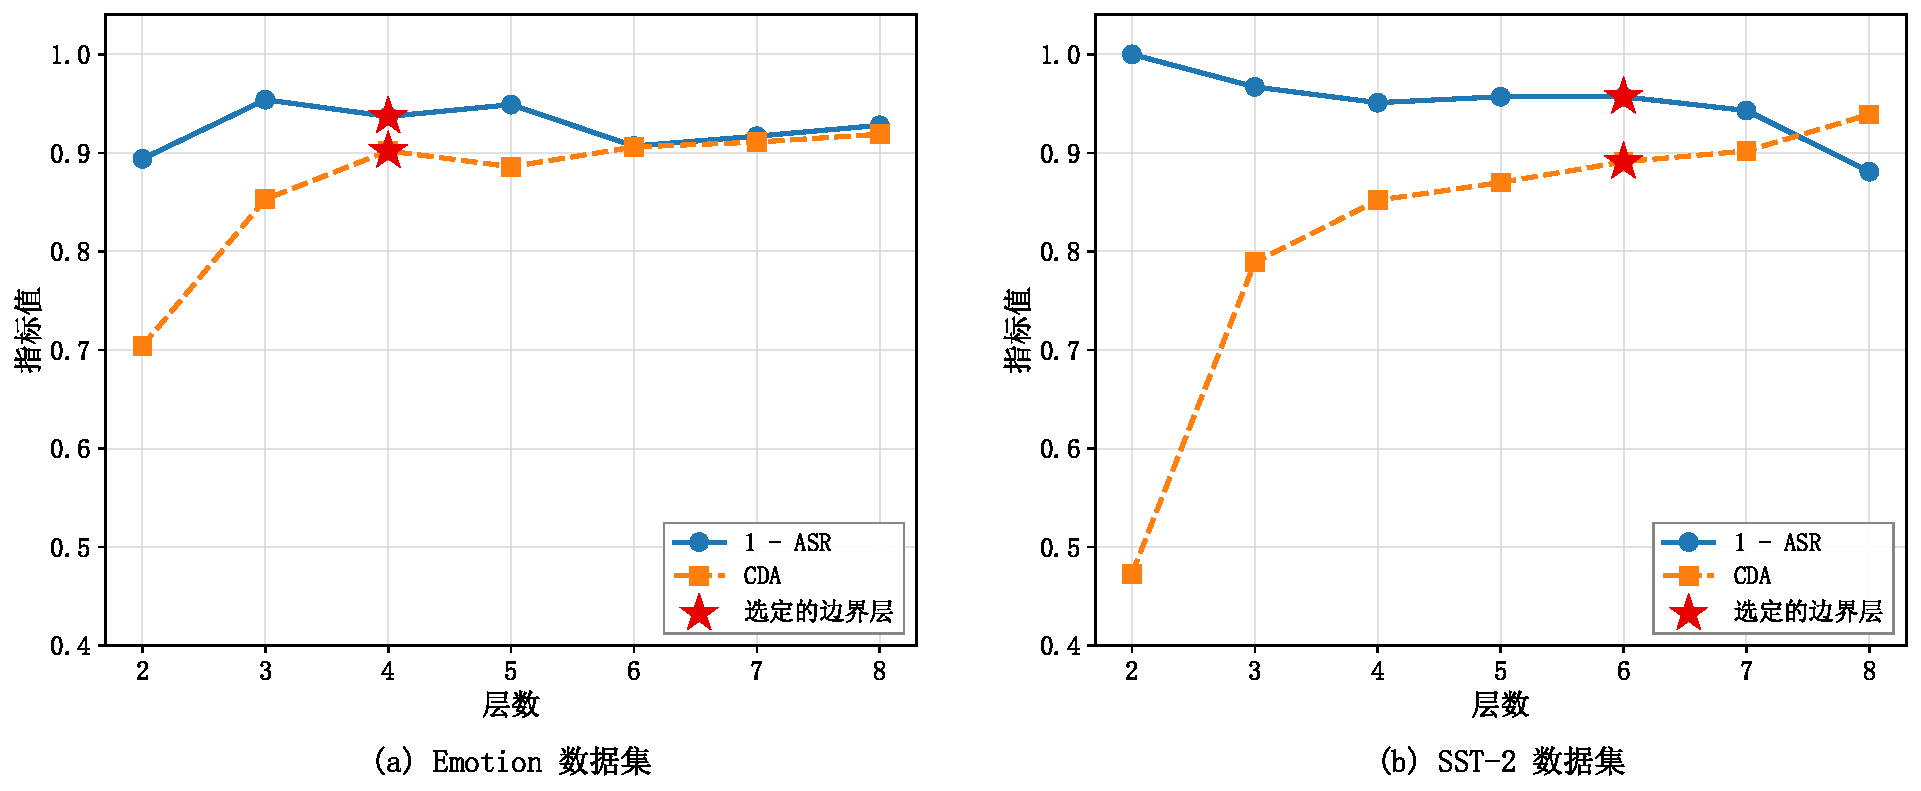
\includegraphics[width=0.95\textwidth]{figures/layer_metric_figure.pdf}
    \caption{不同边界层选择对净化性能（1-ASR和CDA）的影响。星号标记本文方法自动选择的边界层。}
    \label{fig:boundary}
\end{figure}

随着边界层向深层移动，受保护的低层范围增大，CDA随之提升，而1-ASR下降（因参与净化的层减少）。本文基于显著性准则的边界层自动选择机制在Emotion数据集识别出第4层，在SST-2数据集识别出第6层，分别取得ASR 6.3\%/4.4\%和CDA 90.2\%/89.1\%的结果，在ASR降低与CDA保持之间实现了有效的权衡。

\section{面向后门防御即服务的分析}

\subsection{可复用性}

如表~\ref{tab:cls_llama}和表~\ref{tab:gen}所示，ProtoPurify展现了强大的可复用性。后门向量池通过离线模拟使用辅助数据集和已知攻击策略一次性构建，此后可被复用于有效净化所有使用相同架构的目标后门模型，即使这些模型在不同数据集、任务领域和后门攻击下训练。

\subsection{可定制化}

当防御方对后门攻击类型或下游任务有部分了解时，可以利用这些知识提升净化效果。在\textbf{攻击感知}设置中，针对性地使用与目标攻击对应触发器类型的10个后门向量构建原型，相比随机选取10个向量，可以稳定地取得更低ASR和更高CDA。在\textbf{任务感知}设置中，纳入与目标任务相关的向量可分别为Emotion和SST-2数据集带来8.0\%和3.4\%的ASR下降，以及4.0\%和3.3\%的CDA提升。

\subsection{可解释性}

表~\ref{tab:interpretability}分析了ProtoPurify识别出的后门信号$c_i$，揭示了后门更新在模型内部的编码位置和方式。

\begin{table}[htbp]
\centering
\caption{干净模型与受损模型的后门信号分析（均值±标准差）。}
\label{tab:interpretability}
\resizebox{\textwidth}{!}{%
\begin{tabular}{clccc}
\toprule
编号 & 粒度 & 干净模型 & CBA（$\Delta_{\text{CBA}}$） & BadEdit（$\Delta_{\text{BadEdit}}$） \\
\midrule
\multicolumn{5}{l}{\textbf{全局}} \\
1 & 全部参数 & $0.491 \pm 0.147$ & $0.540 \pm 0.102\ (+0.049)$ & $2.108 \pm 0.128\ (+1.617)$ \\
\midrule
\multicolumn{5}{l}{\textbf{子层级}} \\
2 & 自注意力 & $0.561 \pm 0.187$ & $0.565 \pm 0.149\ (+0.004)$ & $2.151 \pm 0.151\ (+1.590)$ \\
3 & MLP & $0.398 \pm 0.006$ & $0.505 \pm 0.030\ (+0.107)$ & $2.051 \pm 0.133\ (+1.653)$ \\
\midrule
\multicolumn{5}{l}{\textbf{投影矩阵级}} \\
4 & $q\_\text{proj}$ & $0.746 \pm 0.017$ & $0.727 \pm 0.019\ (-0.019)$ & $2.204 \pm 0.166\ (+1.458)$ \\
5 & $k\_\text{proj}$ & $0.372 \pm 0.014$ & $0.417 \pm 0.027\ (+0.045)$ & $2.260 \pm 0.125\ (+1.888)$ \\
6 & $v\_\text{proj}$ & $0.374 \pm 0.009$ & $0.414 \pm 0.018\ (+0.040)$ & $2.105 \pm 0.112\ (+1.731)$ \\
7 & $o\_\text{proj}$ & $0.751 \pm 0.012$ & $0.703 \pm 0.039\ (-0.048)$ & $2.034 \pm 0.135\ (+1.283)$ \\
8 & $up\_\text{proj}$ & $0.402 \pm 0.007$ & $0.497 \pm 0.027\ (+0.095)$ & $2.133 \pm 0.126\ (+1.731)$ \\
9 & $gate\_\text{proj}$ & $0.397 \pm 0.005$ & $0.508 \pm 0.023\ (+0.111)$ & $2.077 \pm 0.091\ (+1.680)$ \\
10 & $down\_\text{proj}$ & $0.396 \pm 0.006$ & $0.511 \pm 0.041\ (+0.115)$ & $1.944 \pm 0.136\ (+1.548)$ \\
\bottomrule
\end{tabular}}
\end{table}

结果显示：（1）CBA产生的信号变化较小（$\Delta_{\text{CBA}} = +0.049$），而BadEdit产生的变化约大2个数量级（$\Delta_{\text{BadEdit}} = +1.617$），这一统计特征有助于诊断攻击类型；（2）在子层级，信号增量主要集中在MLP块（+0.107）而非自注意力（+0.004），表明后门更新主要存储在MLP路径中（约27倍）；（3）在注意力投影级，$k\_\text{proj}$和$v\_\text{proj}$呈现小幅正增量，而$q\_\text{proj}$和$o\_\text{proj}$呈现微弱甚至负增量，表明后门倾向于注入存储"内容"的投影矩阵（键和值），而非查询和输出矩阵；所有MLP投影（Up/Gate/Down）均呈现一致的增量。

\subsection{运行时高效性}

ProtoPurify将净化过程分解为一次性离线阶段（阶段一）和每模型服务时阶段（阶段二至四）。服务时流程无需任何模型特定的梯度计算，每个模型的净化时间仅需5--10分钟。相比之下，F/T、NAD和LET等基于训练的基线方法对每个目标模型进行迭代梯度更新，通常需要数百分钟的训练时间。

\section{自适应攻击鲁棒性}

本文考虑了知晓ProtoPurify防御策略的自适应攻击者，该攻击者通过预先放大后门信号$\lambda_i$（Eq.~\eqref{eq:singular_calibrate}）来抵抗原型的净化效果。在原型未泄露设置和原型已泄露设置下，分别使用1.2倍放大因子（更强的放大会导致CDA严重下降至不可用）进行测试。

如表~\ref{tab:adaptive}所示，在两种设置下，ProtoPurify均将ASR保持在10\%以下，且CDA与后门模型相当。这一鲁棒性源于攻击者面临的固有权衡：过强的放大会显著降低CDA，使后门模型失去实用性；而较温和的放大则无法有效抵御ProtoPurify的净化。

\begin{table}[htbp]
\centering
\caption{ProtoPurify对自适应后门攻击的鲁棒性（Llama3-8B）。}
\label{tab:adaptive}
\resizebox{\textwidth}{!}{%
\begin{tabular}{llcccccccccc}
\toprule
\multirow{2}{*}{设置} & \multirow{2}{*}{指标} & \multicolumn{5}{c}{Emotion} & \multicolumn{5}{c}{SST-2} \\
\cmidrule(lr){3-7} \cmidrule(lr){8-12}
& & CBA & BadEdit & VPI & BadNet & 均值 & CBA & BadEdit & VPI & BadNet & 均值 \\
\midrule
原始攻击     & ASR & 1.000 & 0.821 & 0.988 & 1.000 & 0.952 & 1.000 & 0.932 & 1.000 & 1.000 & 0.983 \\
             & CDA & 0.938 & 0.534 & 0.949 & 0.887 & 0.827 & 0.957 & 0.951 & 0.964 & 0.954 & 0.957 \\
\midrule
\multirow{4}{*}{\shortstack{原型未泄露\\（自适应攻击）}}
             & ASR（攻击后）& 1.000 & 0.764 & 0.263 & 0.912 & 0.735 & 1.000 & 0.850 & 0.772 & 0.853 & 0.869 \\
             & CDA（攻击后）& 0.863 & 0.481 & 0.853 & 0.819 & 0.754 & 0.840 & 0.931 & 0.837 & 0.928 & 0.884 \\
             & ASR（净化后）& \textbf{0.095} & \textbf{0.105} & \textbf{0.017} & \textbf{0.125} & \textbf{0.086} & \textbf{0.089} & \textbf{0.152} & \textbf{0.103} & \textbf{0.099} & \textbf{0.111} \\
             & CDA（净化后）& 0.849 & 0.464 & 0.837 & 0.797 & 0.737 & 0.817 & 0.861 & 0.802 & 0.876 & 0.839 \\
\midrule
\multirow{4}{*}{\shortstack{原型已泄露\\（自适应攻击）}}
             & ASR（攻击后）& 0.977 & 0.796 & 0.617 & 0.925 & 0.829 & 1.000 & 0.908 & 0.941 & 0.924 & 0.943 \\
             & CDA（攻击后）& 0.955 & 0.518 & 0.872 & 0.835 & 0.795 & 0.956 & 0.896 & 0.948 & 0.929 & 0.932 \\
             & ASR（净化后）& \textbf{0.107} & \textbf{0.100} & \textbf{0.088} & \textbf{0.016} & \textbf{0.078} & \textbf{0.078} & \textbf{0.142} & \textbf{0.069} & \textbf{0.031} & \textbf{0.080} \\
             & CDA（净化后）& 0.910 & 0.506 & 0.838 & 0.812 & 0.767 & 0.885 & 0.829 & 0.921 & 0.917 & 0.888 \\
\bottomrule
\end{tabular}}
\end{table}

\section{干净模型稳定性}

实用的BDaaS平台必须做到"安全优先"：当提交的模型是良性的（未经中毒训练），净化程序不应降低其干净任务效用。表~\ref{tab:clean}展示了将ProtoPurify应用于干净微调模型前后CDA的变化。

\begin{table}[htbp]
\centering
\caption{干净模型性能（CDA）分析。$\Delta$CDA为应用ProtoPurify前后的绝对变化量。}
\label{tab:clean}
\begin{tabular}{lccc}
\toprule
数据集 & 干净模型CDA & ProtoPurify净化后CDA & $\Delta$CDA \\
\midrule
Emotion & 0.910 & 0.894 & $\pm 0.016$ \\
SST-2   & 0.928 & 0.902 & $\pm 0.026$ \\
\bottomrule
\end{tabular}
\end{table}

ProtoPurify在两个数据集上均仅引入可忽略不计的CDA变化。在无后门诱导的参数更新的情况下，干净模型向量与后门原型的投影很弱，导致净化干预极小，模型效用得以完整保留。

\section{本章小结与全文结论}

\subsection{本章小结}

本章在Llama3-8B和Mistral-7B两种大语言模型上，针对分类和生成两类任务，与6种代表性基线防御方法进行了全面的实验对比。实验结果表明，ProtoPurify在以下方面均取得了优异表现：

\begin{enumerate}[leftmargin=2em]
    \item \textbf{净化效果}：在所有数据集和攻击类型上，ProtoPurify将ASR降低至10\%以下，部分情况下低至1.6\%，同时CDA损失控制在3\%以内，净化-效用综合表现超越所有基线方法。

    \item \textbf{泛化能力}：尽管向量池仅由BadNet一种攻击构建，ProtoPurify仍能有效抵御5种未见攻击；生成任务评估基于分类任务构建的原型，进一步验证了跨领域迁移能力。

    \item \textbf{鲁棒性}：在原型未泄露和原型已泄露两种自适应攻击场景下，ASR均保持在10\%以下。

    \item \textbf{安全性}：{\sloppy 在干净模型上应用ProtoPurify仅引入极小的性能变化，满足BDaaS``安全优先"的要求。\par}
\end{enumerate}

\subsection{全文结论}

本文提出了ProtoPurify，一种面向后门防御即服务（BDaaS）的基于原型表示的大语言模型后门净化方法。ProtoPurify从干净-后门模型对中提取后门原型，通过逐层原型对齐定位受影响的层，并通过以可控净化强度抑制原型对齐分量实现精细化净化。

本文的核心贡献在于：在无需了解触发器、训练数据或下游任务的极少先验假设条件下，实现了可复用、可定制、可解释且运行时高效的后门净化服务。在两种指令微调大语言模型上，针对分类和生成任务的广泛实验表明，ProtoPurify在单触发器、多触发器、无触发器后门设置下，对6种代表性基线方法均取得了优越的净化-效用权衡。

\textbf{局限性与未来工作}：当前ProtoPurify的净化强度$\alpha$是在整个模型层面统一施加的；未来工作可探索在不同子层（如MLP与注意力）或不同投影矩阵之间自适应调整净化强度，以进一步优化净化-效用权衡。此外，随着大语言模型架构的持续演进，如何将ProtoPurify高效扩展至百亿以上参数量的模型也是值得深入探索的方向。


%%----------- 结尾部分 ----------- %%
  \clearpage
  \phantomsection
  \addcontentsline{toc}{chapter}{参考文献}
  \bibliography{ref/refs}   % 参考文献

  % 致谢页

\clearpage
\phantomsection
\addcontentsline{toc}{chapter}{致谢}

\chapter*{致谢}

本文的完成，离不开许多人的帮助与支持，谨在此致以诚挚的感谢。

首先，衷心感谢我的导师王骞教授。在本科毕业设计的整个过程中，王老师给予了我悉心的指导和充分的信任。从研究方向的选定、问题的提炼，到方法的设计与实验的开展，王老师始终以严谨的治学态度和开阔的学术视野引领我前进，使我受益匪浅。

感谢实验室的各位学长学姐和同学。在科研探索的过程中，他们不吝分享宝贵的经验，在我遇到困难时给予及时的帮助，使我能够顺利推进研究工作。

感谢武汉大学计算机学院为我们提供了优良的学习和科研环境。四年的本科学习不仅为我打下了扎实的专业基础，更培养了我独立思考与解决问题的能力。

最后，感谢我的父母和家人。他们的理解、支持与鼓励是我最坚实的后盾，使我得以专注于学业，顺利完成本科阶段的学习与研究。

\vspace{2em}
\begin{flushright}
高嘉鑫\\
2026年5月于武汉大学
\end{flushright}
    % 致谢
  % 附录（已移入第四章实验设置，此文件保留为空）
  % 附录
  \include{pages/null}      % 封底空白页
     

\end{document}